\documentclass{article}

\usepackage{amsmath}
\usepackage{graphicx}
\usepackage{enumitem}

\setlength{\parskip}{\medskipamount}

\title{Advanced Object Oriented Programming and Design\\
\medskip
\large Homework 6 -- Package Design Principles and Metrics}
\author{Abraham Murciano and Daniel Klein}

\begin{document}

\maketitle

\section*{Question 1}

\begin{enumerate}[label=\alph*.]
	\item
		For the package designs given in Figures \ref{q1a-1} and \ref{q1a-2}, the following is known.
		\begin{itemize}
			\item Classes A, B, and C do not contain virtual or pure-virtual functions.
			\item Classes D, G, J, K, L, M, N, and O contain both virtual and pure-virtual functions.
			\item Classes E and H contain both pure-virtual functions and functions that are neither virtual or pure virtual.
			\item Classes F and I contain only virtual functions (not pure virtual).
		\end{itemize}

		\begin{figure}
			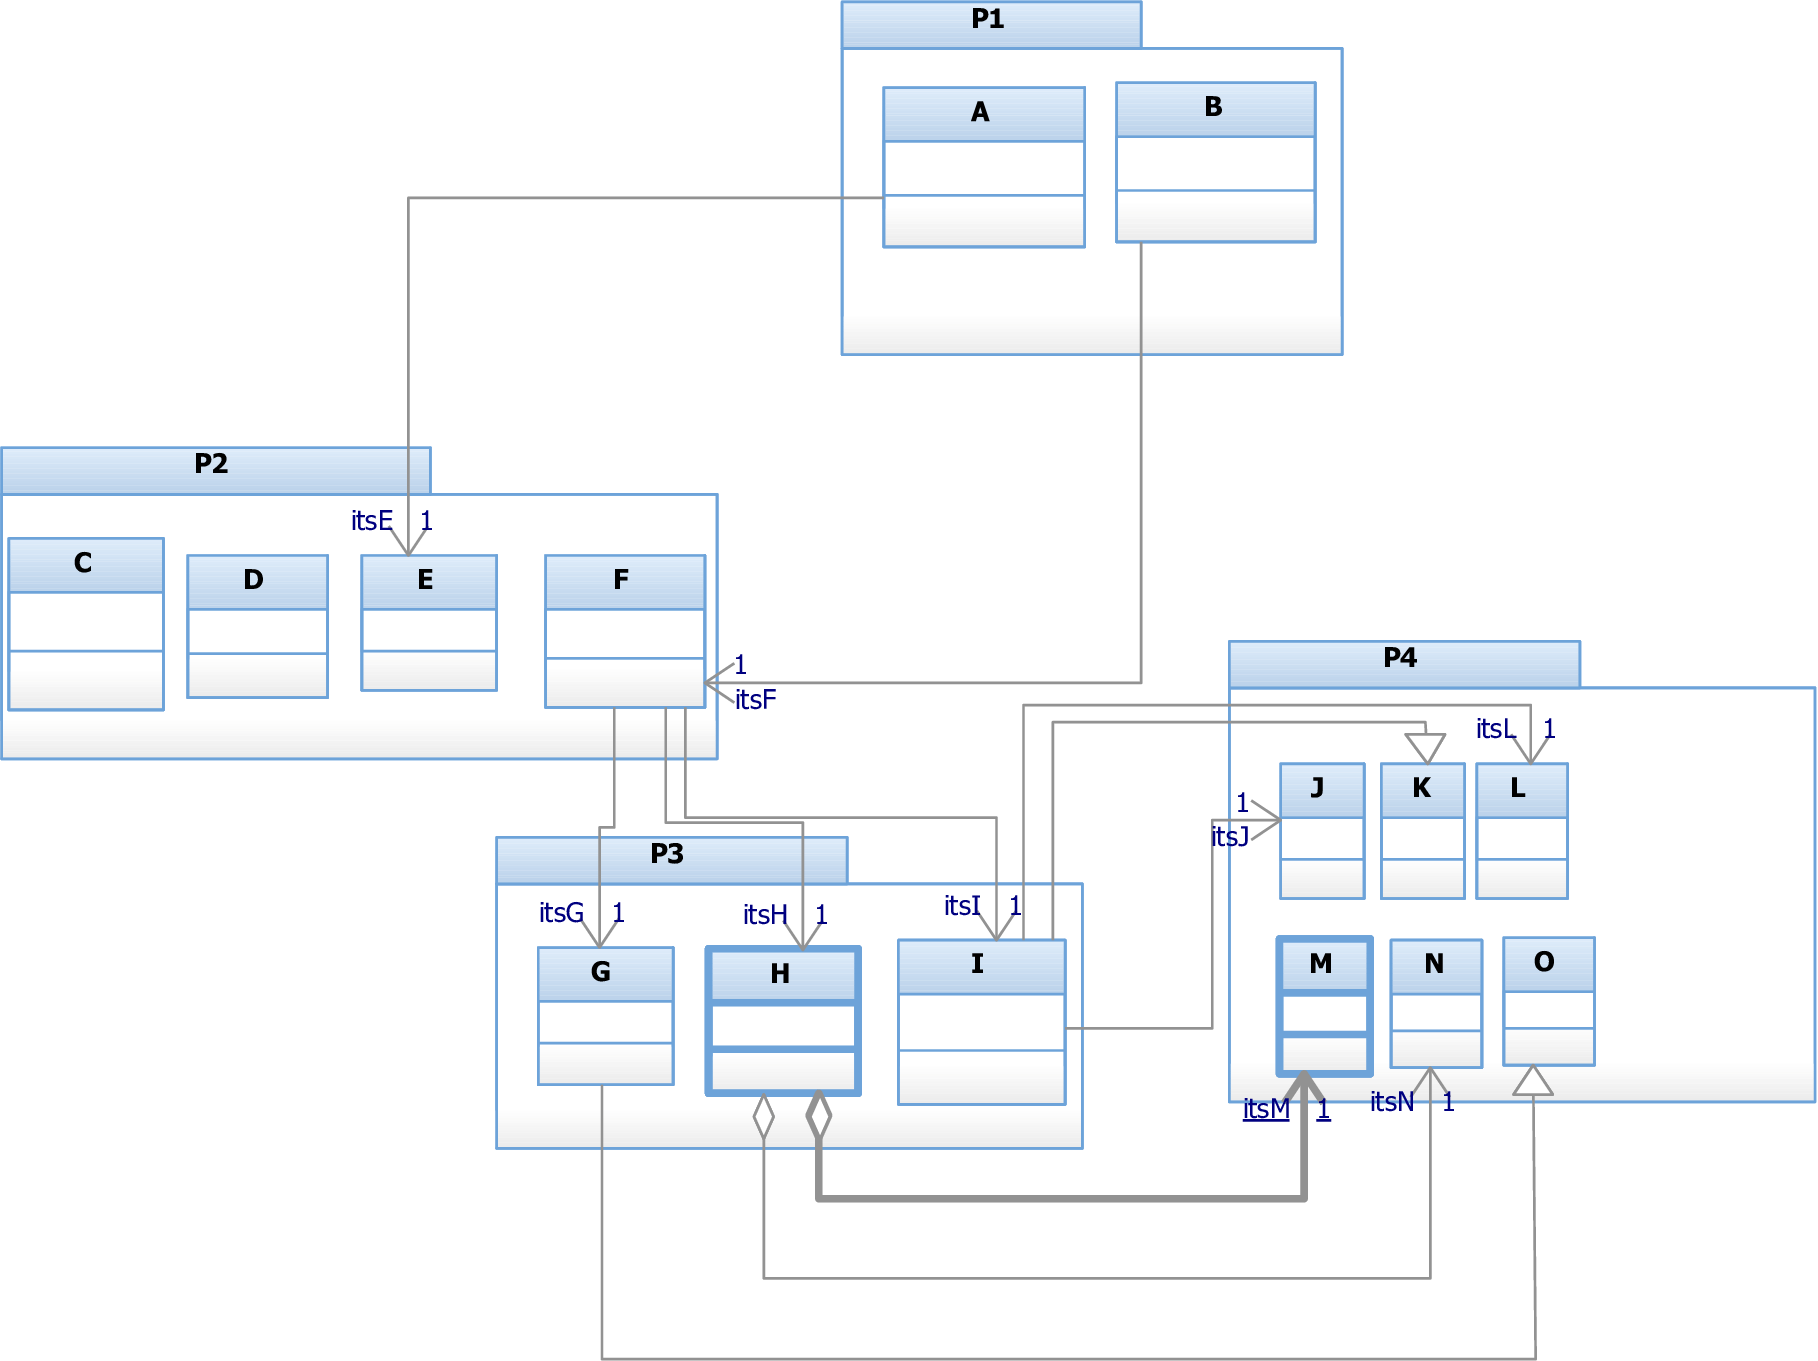
\includegraphics[width=\textwidth]{q1a-1.png}
			\caption{A package design}
			\label{q1a-1}
		\end{figure}
		\begin{figure}
			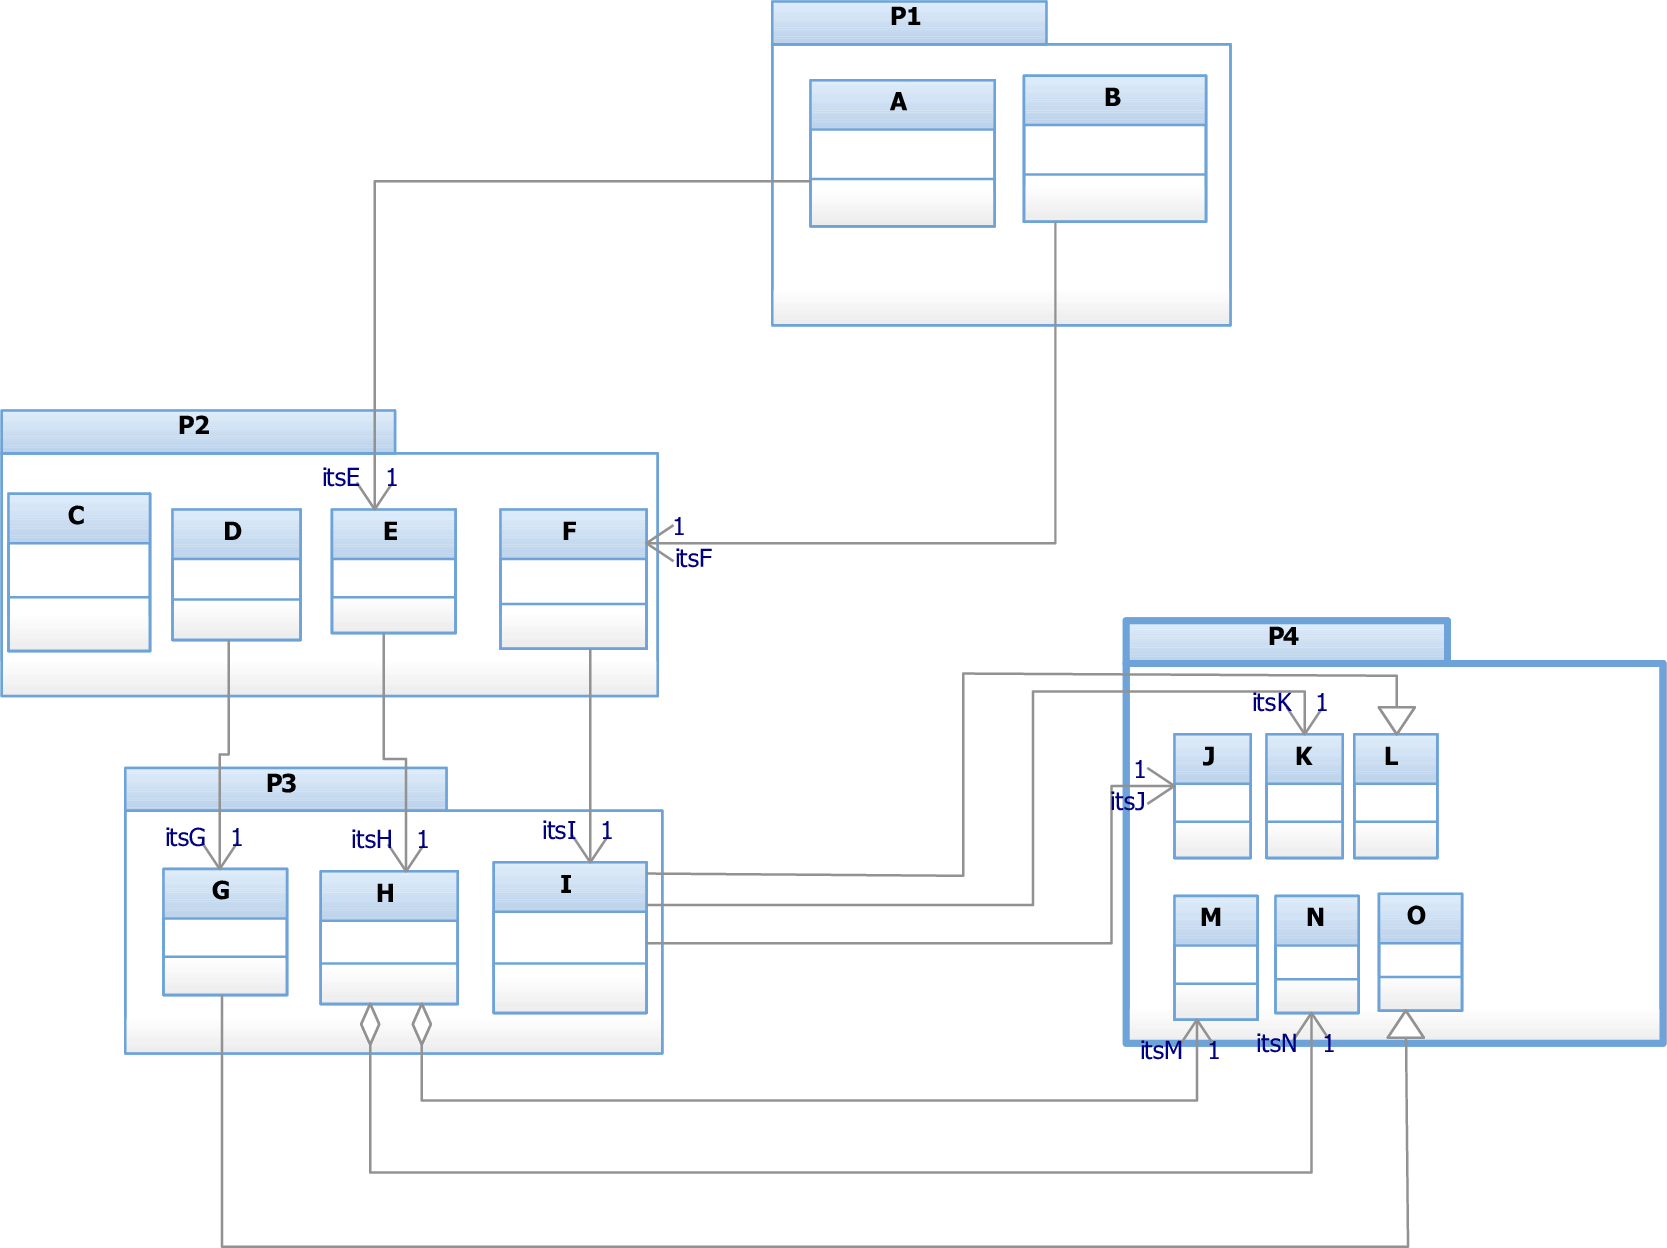
\includegraphics[width=\textwidth]{q1a-2.png}
			\caption{A package design}
			\label{q1a-2}
		\end{figure}

		We are to calculate the following measures for each package, results of which are in tables \ref{q1a-tbl1} and \ref{q1a-tbl2}.
		\begin{align*}
			 & C_a                                                            &  & \text{Number of classes that depend on the package.} \\
			 & C_e                                                            &  & \text{Number of classes that the package depends on.} \\
			 & I = \frac{C_e}{c_a + C_e}                                      &  & \text{Measure of instability.} \\
			 & A = \frac{\# \text{abstract classes}}{\# \text{total classes}} &  & \text{Ratio of abstract classes.} \\
			 & D' = |A+I-1| \\
			 & D = \frac{D'}{\sqrt{2}} \\
		\end{align*}

		\begin{table}[htbp]
			\centering
			\begin{tabular}{||c||c|c|c|c|c|c||}
				\hline
				Class   & \(C_a\) & \(C_e\) & \(I\) & \(A\)         & \(D\)  & \(D'\) \\
				\hline
				\(P_1\) & 0       & 2       & 1     & 0             & 0      & 0 \\
				\(P_2\) & 2       & 3       & 0.6   & 0.5           & 0.0707 & 0.1 \\
				\(P_3\) & 2       & 6       & 0.75  & \(0.\dot{6}\) & 0.2946 & \(1.41\dot{6}\) \\
				\(P_4\) & 3       & 0       & 0     & 1             & 0      & 0 \\
				\hline
			\end{tabular}
			\caption{Values for part a}
			\label{q1a-tbl1}
		\end{table}

		\begin{table}[htbp]
			\centering
			\begin{tabular}{||c||c|c|c|c|c|c||}
				\hline
				Class   & \(C_a\) & \(C_e\) & \(I\)                    & \(A\)         & \(D\)  & \(D'\) \\
				\hline
				\(P_1\) & 0       & 2       & 1                        & 0             & 0      & 0 \\
				\(P_2\) & 2       & 3       & 0.6                      & 0.5           & 0.0707 & 0.1 \\
				\(P_3\) & 1       & 6       & \(0.\dot{8}5714\dot{2}\) & \(0.\dot{6}\) & 0.3705 & \(1.\dot{5}2389\dot{9}\) \\
				\(P_4\) & 3       & 0       & 0                        & 1             & 0      & 0 \\
				\hline
			\end{tabular}
			\caption{Values for part b}
			\label{q1a-tbl2}
		\end{table}

	\item
		The design in figure \ref{q1a-1} violates the Stable Dependencies Principle because \(P_2\) depends on \(P_3\) which has a higher instability than \(P_2\).
\end{enumerate}


\section*{Question 2}

\begin{enumerate}[label=\alph*.]
	\item
		We are to divide classes \(A\) through \(J\) into packages. The following information is given regarding the classes.
		\begin{itemize}
			\item Client 1 reuses all the classes.
			\item Client 2 reuses classes \(A\), \(B\) and \(C\).
			\item Client 3 reuses classes \(A\) through \(F\).
			\item Classes \(A\) and \(D\) are written in Java, classes \(E\) through \(H\) are written in Python, and classes \(I\) and \(J\) are in C++.
			\item A past feature update required changing classes \(G\) through \(J\).
			\item Classes \(G\) and \(H\) and classes \(I\) and \(J\) are two alternatives that implement the same pair of interfaces. A reusing project may choose to import either the first or the second couple.
		\end{itemize}

		We decide to split the classes into the following packages.

		\begin{align*}
			P_1 & = (A, B, C) \\
			P_2 & = (D, E, F) \\
			P_3 & = (G, H) \\
			P_4 & = (I, J)
		\end{align*}

		The reason why the classes are split up into smaller packages is so that each client only uses the packages containing classes that they need. This is in accordance with the Reuse/Release Equivalence Principle.

		The reason we grouped certain classes in the same package is because they are always reused together by the clients. This follows the Common Reuse Principle.

		According to the Common Closure Principle, classes G through J should be in the same package because they are changed together. However, since they are alternative implementations of the same interface, we choose to keep them separate so that they can be reused individually in accordance to the Common Reuse Principle.

	\item
		Assume the same dependencies between packages (ignoring the actual class names) as in figure \ref{q1a-1}. If classes \(A\) and \(B\) are changed, only package \(P_1\) needs to be redistributed, and no other package needs to be changed, since nothing depends on \(P_1\).

\end{enumerate}

\end{document}